\section{Network Manipulation and Analysis}
\label{sec:part3}
Two tasks are addressed, one from each of the two required clusters: Link Prediction, an analytical task, and Spreading~2, a custom diffusion model for the manipulation cluster, for which the course's standard epidemic models serve only as a baseline.

\subsection{TASK 1: LINK PREDICTION}
Following Liben-Nowell \& Kleinberg~\cite{linkpred}, the edges are split into a training set (80\%) and a held-out test set (20\%), and node pairs are scored on the training graph with four classical unsupervised predictors: Common Neighbors (CN), Jaccard, Adamic--Adar (AA) and Preferential Attachment (PA). Accuracy is measured as in the reference paper: the candidate pairs, the held-out test edges (positives) plus a large pool of random non-edges (negatives), in a strongly imbalanced $1{:}50$ setting that mimics the paper's realistic ``few true links among many candidates'' scenario, are ranked by each predictor; the top-$n$ pairs are taken ($n=2{,}000$, the number of positives) and the fraction that are real edges gives precision@$n$. The headline figure, exactly as in the paper, is the improvement factor over a random predictor, whose baseline precision@$n$ equals the prevalence ($0.020$); AUC-ROC is reported as a complementary modern metric (Table~\ref{tab:lp}).

\begin{table}[h]
  \centering\small
  \caption{Link prediction accuracy in the paper's imbalanced ($1{:}50$) ranking setting. ``$\times$rand'' is the improvement factor over a random predictor (baseline precision@$n = 0.020$)}
  \label{tab:lp}
  \begin{tabular}{lccc}
    \toprule
    Predictor & P@$n$ & $\times$rand & AUC \\
    \midrule
    Common Neighbors        & 0.402 & 20.5 & 0.939 \\
    Jaccard                 & 0.373 & 19.0 & 0.923 \\
    Adamic--Adar            & \textbf{0.419} & \textbf{21.4} & \textbf{0.943} \\
    Preferential Attachment & 0.176 & 9.0  & 0.816 \\
    \bottomrule
  \end{tabular}
\end{table}

\noindent All four predictors beat the random baseline by a wide margin, reproducing the paper's central finding. The three neighborhood-based scores are the strongest ($\approx 19$--$21\times$ random, AUC $\approx 0.92$--$0.94$), with Adamic--Adar best, consistent with the reference paper, since weighting shared neighbors by their (inverse) degree rewards specific, low-degree common contacts. Preferential Attachment, which ignores common neighbors and only multiplies the endpoint degrees, lags clearly behind ($9.0\times$ random, AUC $0.816$): in this network proximity matters far more than mere popularity. Unlike a balanced $1{:}1$ evaluation, the realistic imbalance brings precision@$n$ down to $\approx 0.4$, the true difficulty of the task stressed by the paper, while the $\sim\!20\times$ improvement factors quantify how much structure each score exploits over chance.

\subsection{TASK 2: SPREADING 2 -- a custom diffusion model}

\subsection{Baseline}
As a reference, the standard SI, SIS, SIR and Threshold models are first simulated with NDlib on the real network and, for SIR, on ER/BA graphs of comparable size, varying parameters and seeds (Figures~\ref{fig:diffmodels}--\ref{fig:diff}). SI saturates to full infection, SIS settles at an endemic equilibrium ($\approx 0.99$), SIR peaks at $\approx 0.90$ around iteration~8, and the Threshold model triggers an almost immediate total cascade, unsurprising given the very high average degree ($222$). Across topologies the SIR curves almost overlap: on such a dense graph diffusion is fast and near-total everywhere, the real network even peaking marginally lower because its redundant intra-community edges are ``wasted'' on already-infected neighbors.

\begin{figure}[h]
  \centering
  
\includegraphics[width=\linewidth]{figures/diffusion_models_real.png}
  \caption{Baseline: SI, SIS, SIR and Threshold models on the real network.}
  \label{fig:diffmodels}
\end{figure}

\begin{figure}[h]
  \centering
  
\includegraphics[width=\linewidth]{figures/diffusion_sir_compare.png}
  \caption{Baseline: SIR diffusion, real network vs ER vs BA.}
  \label{fig:diff}
\end{figure}

The assignment's requirement to vary both model parameters and initial conditions is made explicit on the SIR model (Figure~\ref{fig:sir-param}). Raising the infection rate $\beta$ from $0.002$ to $0.02$ makes the epidemic peak higher and much earlier (from $\approx0.77$ around iteration~20 to $\approx0.93$ around iteration~6), yet all curves converge to the same tail: on this dense, small-world graph $\beta$ governs the speed of the outbreak, not its final size. The initial seed fraction, by contrast, is almost irrelevant, varying it from $1\%$ to $20\%$ of the nodes leaves the SIR trajectory practically unchanged (only the first few iterations differ). This is the sharpest contrast with the custom cascade below (Figure~\ref{fig:game-thr}): for a simple contagion on a dense graph how many seeds hardly matters, whereas for the coordination cascade which nodes are seeded is decisive.

\begin{figure}[h]
  \centering
  
\includegraphics[width=0.49\linewidth]{figures/diffusion_sir_beta.png}\hfill
  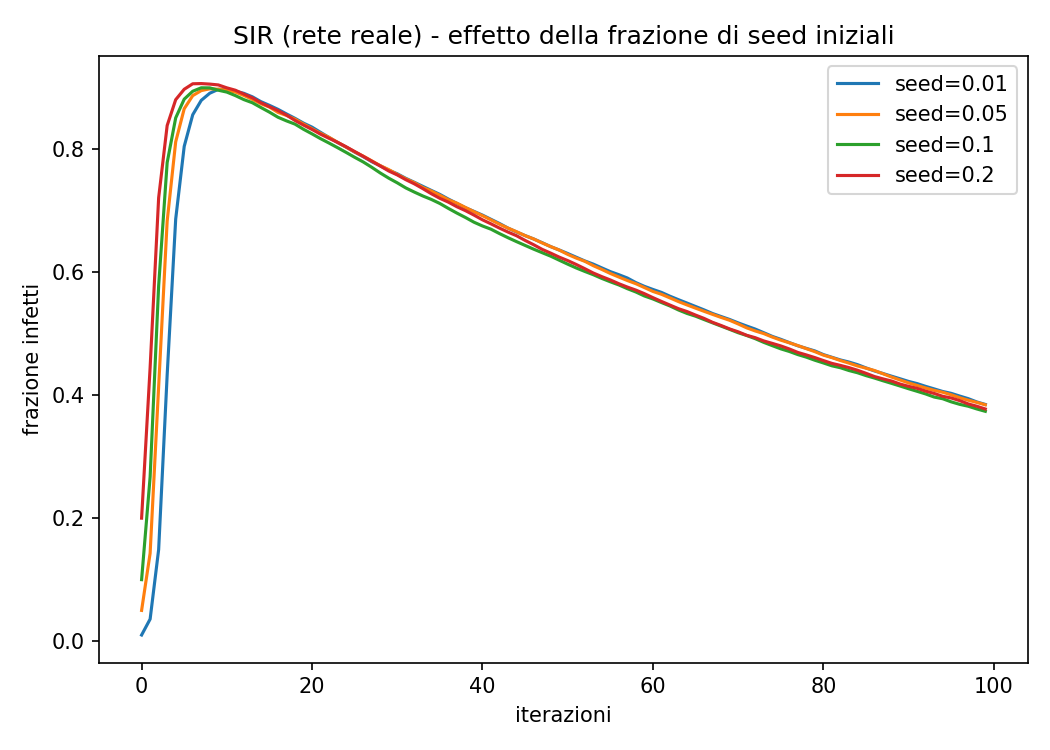
\includegraphics[width=0.49\linewidth]{figures/diffusion_sir_seeds.png}
  \caption{Baseline SIR on the real network. Left: varying the infection rate $\beta$ raises and anticipates the peak but leaves the final size unchanged. Right: varying the initial seed fraction ($1$--$20\%$) barely affects the trajectory.}
  \label{fig:sir-param}
\end{figure}

\subsection{Custom model}
For the manipulation task a bespoke, deterministic diffusion model is implemented directly in Python rather than through NDlib, to retain full control over its threshold update rule, with NDlib reserved for the baseline above, based on a two-player coordination game~\cite{granovetter,kleinberg} played on every edge: each account chooses behavior A or B and gains from matching its neighbors (payoff $a$ if both choose A, $b$ if both B, $0$ otherwise). A node $v$ adopts A iff the fraction of its A-neighbors is at least $q=b/(a+b)$; a seed set is hard-wired to A and the cascade is deterministic. The model is then made group-aware, its ad-hoc, novel ingredient, by down-weighting coordination across group boundaries by a factor $\omega\in[0,1]$, so $v$ adopts A iff
\[
\frac{A_{\mathrm{in}} + \omega\,A_{\mathrm{out}}}{D_{\mathrm{in}} + \omega\,D_{\mathrm{out}}}\;\ge\;q,
\]
where $A_{\mathrm{in}}/A_{\mathrm{out}}$ ($D_{\mathrm{in}}/D_{\mathrm{out}}$) are the active (total) neighbors inside/outside $v$'s group. $\omega=1$ recovers the plain model; $\omega<1$ models homophilous coordination (accounts coordinate more readily with same-group peers). The grouping deliberately exploits both kinds of information the task calls for: network topology, the Louvain community structure (barriers experiment), and genuine external semantic information, a topical label attached to each of the $14{,}598$ accounts with posts, obtained by TF-IDF vectorizing the text of their posts and KMeans-clustering them into ten topical groups (semantic experiment). The model is analyzed by varying both its parameters ($q$, $\omega$) and the initial conditions (the seed set).

\subsection{Seed placement vs.\ critical threshold}
At equal seed budget ($k=150$, $1\%$ of nodes), the largest threshold still yielding a global cascade ($q^{*}$) is $\approx0.05$ for random seeds, $\approx0.20$ for high-degree hubs and $\approx0.25$ for seeds concentrated in a single community (Figure~\ref{fig:game-thr}). Hubs trigger global adoption at $4$--$5\times$ higher thresholds: which nodes are activated matters far more than how many, linking the centrality analysis of Section~\ref{sec:analysis} to diffusion.

\subsection{Communities as barriers}
Seeding an entire community and increasing $q$, the spill-over into the other communities exhibits a sharp transition around $q\approx0.41$: it stays at $100\%$ for $q\le0.40$ but collapses to $<2\%$ at $q=0.45$, where the seeded community remains fully adopted while the others stay at $0$--$12\%$ (Figure~\ref{fig:game-bar}). This empirically confirms the theoretical result that a sufficiently dense cluster (density $>1-q$) halts a cascade: the topical communities of Section~\ref{sec:cd} act as diffusion barriers.

\subsection{Homophilous coordination along topical lines}
The novel, semantic ingredient uses the text-derived topical groups. Fixing $q=0.40$ and seeding an entire topical group, the cross-topic weight $\omega$ has a striking effect (Figure~\ref{fig:game-omega}): while cross-topic coordination stays fairly symmetric ($\omega\ge0.5$) the cascade still floods the whole network ($100\%$ spill-over), but once same-topic coordination is preferred strongly enough ($\omega\le0.25$) the spill-over collapses, to $8.3\%$ ($2.3\%$ at $\omega=0.1$) for the largest topical group and to just $3.9\%$ ($0.6\%$ at $\omega=0.1$) for a smaller, tighter one, confining the cascade to the seeded group. Repeating the sweep for a second seeded group (varying the initial conditions) confirms the pattern, the denser group forming the stronger barrier. Homophilous coordination along topical lines is thus enough to turn the semantic structure into a near-perfect barrier, a behavioral counterpart to the topical echo chambers studied in Section~\ref{sec:open}.

\begin{figure}[h]
  \centering
  
\includegraphics[width=\linewidth]{figures/game_threshold_seeding.png}
  \caption{Custom cascade: final adoption vs.\ threshold $q$ for three seeding strategies (equal budget)}
  \label{fig:game-thr}
\end{figure}

\begin{figure}[h]
  \centering
  
\includegraphics[width=0.49\linewidth]{figures/game_community_barriers.png}\hfill
  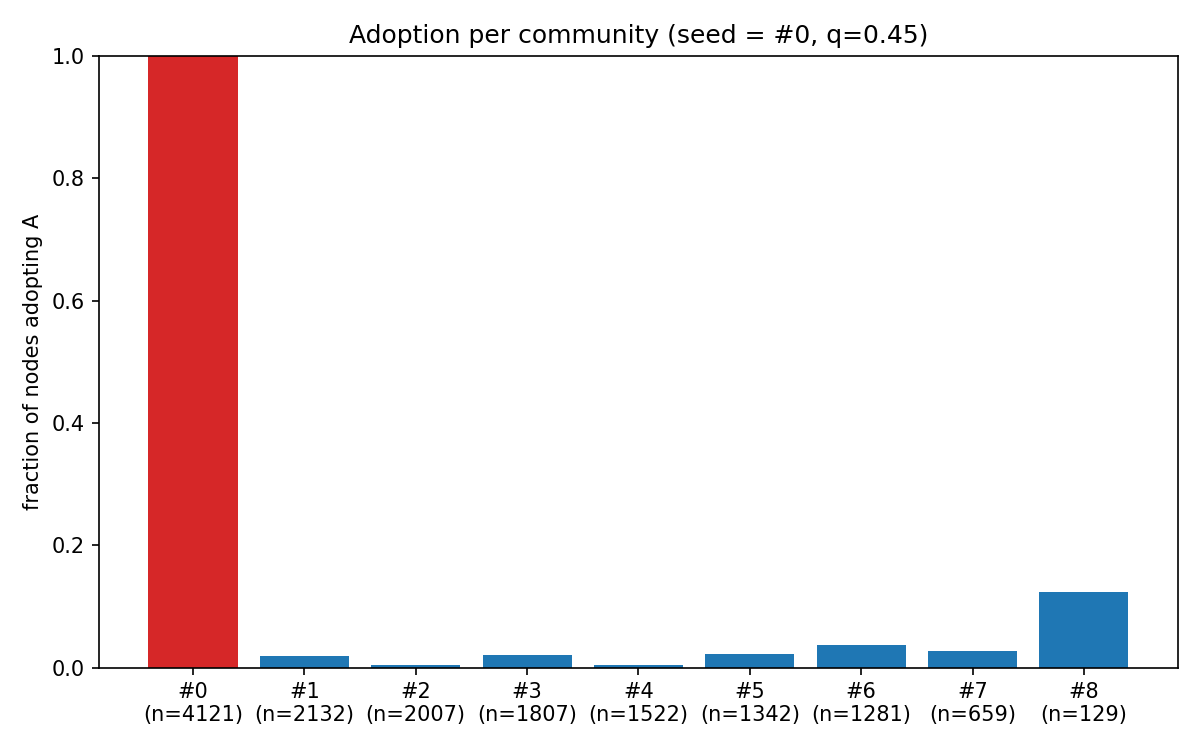
\includegraphics[width=0.49\linewidth]{figures/game_community_barriers_detail.png}
  \caption{Communities as diffusion barriers. Left: the spill-over outside the seeded community stays at $100\%$ for $q\le0.40$ and collapses sharply once $q$ exceeds $\approx0.41$. Right: at $q=0.45$ the cascade stays confined to the seeded community (red).}
  \label{fig:game-bar}
\end{figure}

\begin{figure}[h]
  \centering
  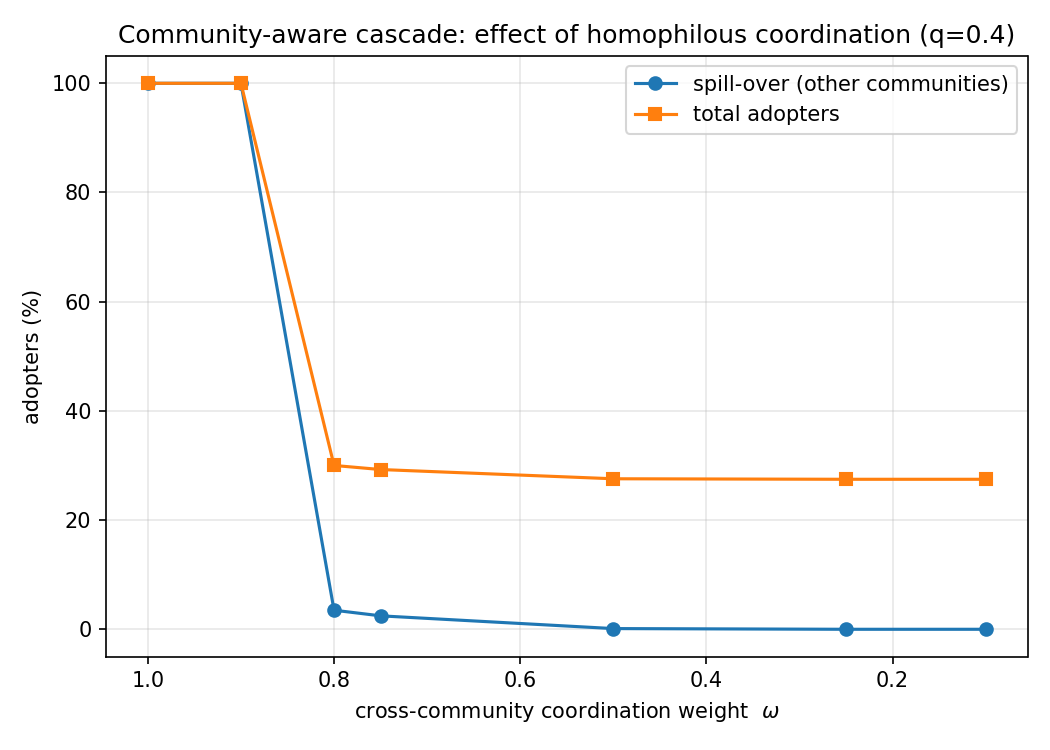
\includegraphics[width=\linewidth]{figures/game_custom_omega.png}
  \caption{Custom semantic model: spill-over into the other topical groups as the cross-topic coordination weight $\omega$ decreases, for two seeded topical groups ($q=0.40$)}
  \label{fig:game-omega}
\end{figure}
